\documentclass[11pt,oneside, a4paper]{article}
\usepackage{titlesec}
\usepackage{graphicx}
\usepackage{color}
\usepackage[nottoc]{tocbibind}
\usepackage[titletoc]{appendix}
\usepackage{amsthm}
\usepackage{titlesec}
\usepackage{tikz}
\usepackage{caption}
\usepackage{subcaption}
\usepackage[backend=bibtex, style=ieee, bibencoding=utf8]{biblatex}
\usepackage{amssymb}
\usepackage[utf8]{inputenc}
\usepackage[DIV=14,BCOR=2mm,headinclude=true,footinclude=false]{typearea}

\definecolor{keywordcolor}{rgb}{0.7, 0.1, 0.1}   % red
\definecolor{commentcolor}{rgb}{0.4, 0.4, 0.4}   % grey
\definecolor{symbolcolor}{rgb}{0.0, 0.1, 0.6}    % blue
\definecolor{sortcolor}{rgb}{0.1, 0.5, 0.1}      % green
\definecolor{tacticcolor}{rgb}{0.0, 0.1, 0.6}
\definecolor{background}{gray}{0.95}

\usepackage{listings}
\def\lstlanguagefiles{lstlean.tex}
\lstset{
  language=lean, 
  mathescape=true, 
  breaklines=true,
}
\newcommand{\dollar}{\mbox{\textdollar}}

\makeatletter
\DeclareCaptionFormat{alsoempty}{%
  #1\if\relax\expandafter\noexpand\lst@caption\else#2#3\fi}
\makeatother
\captionsetup[lstlisting]{format=alsoempty}

\newcommand\notes[1]{\textcolor{red}{#1}}

\theoremstyle{definition}
\newtheorem{definition}{Definition}[section]

\theoremstyle{definition}
\newtheorem{lemma}{Lemma}[section]

\addbibresource{refs.bib}

\begin{document}

% Title Page
% \thispagestyle{empty}

\begin{center}

Vrije Universiteit Amsterdam

\vspace{1cm}

\includegraphics[height=28mm]{logo.png}

\vspace{1cm}

{\Large Bachelor Thesis}

\vspace*{1.5cm}

\rule{.9\linewidth}{.6pt}\\[0.4cm]
{\huge \bfseries Verifying AVL Trees\par}
{\huge \bfseries in Lean\par}\vspace{0.4cm}
\rule{.9\linewidth}{.6pt}\\[1.5cm]

\vspace*{2mm}

{\Large
\begin{tabular}{l}
{\bf Author:} ~~Sofia Konovalova ~~~~ (2635220)
\end{tabular}
}

\vspace*{1.5cm}

\begin{tabular}{ll}
{\it 1st supervisor:}   & ~~Jasmin Blanchette \\
{\it daily supervisor:} & ~~Jannis Limperg ~~~~ \\
{\it 2nd reader:}       & ~~Alexander Bentkamp
\end{tabular}

\vspace*{2cm}

\textit{A thesis submitted in fulfillment of the requirements for\\ the VU Bachelor of Science degree in Computer Science }

\vspace*{1cm}

\today\\[4cm] % Date

\end{center}

% \tableofcontents

% \newpage 

%\begin{abstract}
	%lorem ipsum
%\end{abstract}

% \section{Introduction}

%FIRST DRAFT%
% \section{Lean Theorem Prover}
% The Lean Theorem Prover is a proof assistant based on dependent type theory with inductive families and universe polymorphism \cite{inductive_families}. The language contains dependent function types and inductive types.

In simple type theory, every expression has an associated type. Lean's dependent type theory extends simple type theory by having types themselves be types. Types can also be built from other types \cite{lean:manual}.  

\begin{lstlisting}
  /- simple types -/
  constant m : nat
  constant b : bool
  /- types from other types -/
  constant g : nat → nat
  #check g m -- nat
\end{lstlisting}

The code above shows some examples of types. The constant \lstinline{m} is a natural number type, and \lstinline{b} is a boolean type. The constant \lstinline{g} is a type of function from a natural number to another natural number. This can be applied to any other type too; if \lstinline{α} and \lstinline{β} are types, then \lstinline{α → β} is the type of functions from \lstinline{α} to \lstinline{β}.

With dependent type theory, types can depend on values. For example, \lstinline{list α} depends on \lstinline{α}, which helps differentiate between lists of different types. If we want to define a function which adds a new value to the list, the function would be polymorphic as its expected to function the same way with a \lstinline{bool}, \lstinline{nat} or any other \lstinline{α} type list. A function to add a new element to the list would have a type \lstinline{∀ α, list α → list α}, which is an example of a dependent function type, as the outcome of the function is dependent on the type \lstinline{α} of the parameters.\todo{change to a different example}

In Lean, an inductive type is has zero or more constructors, and each constructor specifies a way of building an inhabitant of the type. 

\begin{lstlisting}
inductive foo (a : α) : Sort u
| constructor₁: Π (b : β₁) → foo
| constructor₂: Π (b : β₂) → foo
\end{lstlisting}

An inductive type may be recursive if the arguments within the constructors \lstinline{(b₁ : β₁)} refer to the inductive type itself \cite{lean:reference}.


%FIRST DRAFT%
% \section{AVL Trees and Operations}
% This section defines binary search trees and AVL trees, as well as operations such as key search, rotation and deletion with the corresponding Lean formalization.

\subsection{Binary Search Trees}
A binary search tree (BST) (also called an ordered tree) is a tree data structure where each node has at most two children, referred to as the \textit{left child} and \textit{right child}. A node also has a key and a value for storing information.

To formalize binary trees, I defined an inductive type \lstinline{btree}.

\begin{lstlisting}[caption=\empty]
inductive btree (α : Type u)
| empty {} : btree
| node (l : btree) (k : nat) (a : α) (r : btree) : btree
\end{lstlisting}

In this definition, there are two constructors: one for an empty tree, and one for a node, with two children, a key and a node value. There is no leaf constructor, as a leaf is a node with no children, which can be easily defined with the \lstinline{node} constructor.

From there, I defined a function to search for a key in a tree. The purpose of the function is to verify that a key exists in a tree; therefore, it doesn't matter in which subtree it is located in, as long as it is in one of them.

\begin{lstlisting}[caption=\empty]
def bound (x : nat) : btree α → bool
| btree.empty := ff
| (btree.node l k a r) :=
  x = k ∨ bound l ∨ bound r
\end{lstlisting}

All nodes in a binary search tree must have the \textit{binary search property}.

\begin{definition}[Binary Search Property]
  \label{def:bst_property}
  Given any node N in a binary search tree, all the keys in the left subtree of N are smaller than the key of N, and all keys in the right child subtree are greater than the 
  key of N.
\end{definition}

The binary search property is formalized with two definitions. \lstinline{forall_keys} describes the relationship between a key and a tree - for all the keys that exist in a tree, there is some relationship between the input key and the tree keys. 

\begin{lstlisting}[caption=\empty]
def forall_keys (p : nat → nat → Prop) (k : nat) (t : btree α) : Prop :=
  ∀ k', bound k' t → p k k'
\end{lstlisting}

The definition for \lstinline{ordered} uses the \lstinline{forall_keys} definition to formalize the binary search property. A tree is ordered only if the children are ordered and the \lstinline{forall_keys} relationship holds.

\begin{lstlisting}[caption=\empty]
def ordered : btree α → Prop
| btree.empty := tt
| (btree.node l k a r) :=
  ordered l ∧ ordered r ∧ (forall_keys (>) k l) ∧ (forall_keys (<) k r)
\end{lstlisting}

Due to the binary search property, operations such as lookup can be done recursively. For traversal, it is possible to compare every key to another as a total preorder relation is required for binary search trees. When traversing the tree, the input key is compared with the current node, and the left subtree or the right subtree is then recursively traversed depending on if the input key is smaller or larger than its root, respectively.

Listing \ref{lst:def_lookup} shows the \lstinline{lookup} function - a key is searched for in a tree, traversing the tree as stated previously and the node data is returned if a key is located.

\begin{lstlisting}[caption=\empty, label={lst:def_lookup}]
def lookup (x : nat) : btree α → option α
| btree.empty := none
| (btree.node l k a r) :=
  if x < k then lookup l
  else if x > k then lookup r
  else a
\end{lstlisting}

\subsection{AVL Trees}
An AVL tree \cite{avl:original} is a self-balancing binary search tree, where the absolute value of the height difference between two child subtrees is no more than one. 
This may also be described by the \textit{balancing factor}.

\begin{definition}[Tree height]
  \label{def:height}
  The height of a node in a tree is the maximal number of edges from that node to a leaf.
\end{definition}

\begin{definition}[Balancing factor]
  \label{def:balancing_factor}
  The balancing factor of any node is defined to be the height difference of its two child subtrees.
\end{definition}

In Lean, the definitions \lstinline{height} and \lstinline{balanced} are done per Definitions \ref{def:height} and \ref{def:balancing_factor}.

\begin{lstlisting}
def height : btree α → nat
| btree.empty := 0
| (btree.node l k a r) :=
  1 + (max (height l) (height r))

def balanced : btree α → bool
| btree.empty := tt
| (btree.node l k a r) :=
  if height l ≥ height r 
    then height l ≤ height r + 1
    else height r ≤ height l + 1
\end{lstlisting}

The process of looking up a node or searching for a key is the same as in BSTs. 

During insertion and deletion, however, it is more complicated. In self-balancing trees, re-balancing actions are not performed arbitrarily, but after operations such as insertion and deletion that may change the structure of the tree. In the case of AVL trees, a tree may become left-heavy or right-heavy after these actions, after which the tree is re-balanced with rotations. Left-heaviness can be fixed with a simple right rotation; right-heaviness with a simple left rotation. 

A tree \lstinline{t} being left-heavy means that the left subtree's height is $n+2$ given height of the right subtree $n$; similarly, in a right-heavy tree, given the height $n$ of the left subtree, the height of the right subtree is $n+2$. The definitions presented further closely follow \cite{textbook:discrete_computer}. The definition for \lstinline{right_heavy} is mirrored.

\begin{lstlisting}
def left_heavy : btree α → bool
| btree.empty := ff
| (btree.node btree.empty k a r) := ff
| (btree.node (btree.node ll lk la lr) k a r) :=
  (height ll ≥ height lr) ∧ (height ll ≤ height lr + 1) ∧
  (height lr ≥ height r) ∧ (height r + 1 = height ll)
\end{lstlisting}

\begin{figure}[!ht]
  \begin{subfigure}[c]{0.3\textwidth}
    \centering
    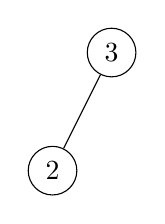
\begin{tikzpicture}
      \node[circle,draw](z){3}
        child {
          node[circle,draw]{2}
            child[missing]
            child[missing]
        }
        child[missing];
      \end{tikzpicture}
  \end{subfigure}%
  \begin{subfigure}{0.3\textwidth}
    \centering
    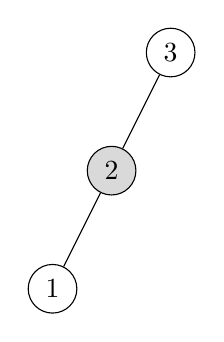
\begin{tikzpicture}
      \node[circle,draw](z){3}
        child {
          node[circle,draw,fill=gray!30]{2}
            child {
              node[circle,draw]{1}
                child[missing]
                child[missing]
            }
            child[missing]
        }
        child[missing];
      \end{tikzpicture}
  \end{subfigure}%
  \begin{subfigure}[c]{0.3\textwidth}
    \centering
    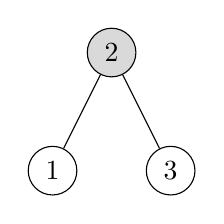
\begin{tikzpicture}
      \node[circle,draw,fill=gray!30](z){2}
        child{
          node[circle,draw]{1}
            child[missing]
            child[missing]
        }
        child{
          node[circle,draw]{3}
            child[missing]
            child[missing]
        };
    \end{tikzpicture}
  \end{subfigure}
  \caption{}
  \label{fig:rotation}
\end{figure}

An example of a simple right rotation is shown in Figure \ref{fig:rotation}. After the node with the key of 1 gets inserted, the tree becomes left-heavy, which can be fixed with a right rotation. The direct ancestor of the newly inserted node with the key of 2 becomes the new root of the tree, and the ancestor of the new root moves to the right. The result is a balanced tree, with order and the keys preserved.

\begin{lstlisting}
def simple_right : btree α → btree α
| btree.empty := btree.empty
| (btree.node (btree.node ll lk la lr) k a r) := 
    btree.node ll lk la (btree.node lr k a r)
| (btree.node l k a r) := btree.node l k a r
\end{lstlisting}

Compound rotations are performed when after a simple rotation the tree is still unbalanced. If after a left rotation, the tree is becomes left-heavy then a right rotation is done to fix the heaviness. The definition for \lstinline{rotate_left} is mirror. \todo{maybe add a figure here for compound rotations?}

\begin{lstlisting}
def rotate_right : btree α → btree α
| btree.empty := btree.empty
| (btree.node l k a r) :=
  match l with
  | btree.empty := (btree.node l k a r)
  | (btree.node ll lk la lr) :=
    if height ll < height lr 
      then simple_right (btree.node (simple_left l) k a r)
      else simple_right (btree.node l k a r)
  end 
\end{lstlisting}

The insertion definition makes use of the definitions of heaviness and rotations to insert a node into a tree while retaining balance. If insertion creates a left-heavy tree, then a right rotation is done, and if it creates a right-heavy tree, then a left rotation is done.

\begin{lstlisting}
def insert (x : nat) (v : α) : btree α → btree α
| btree.empty := btree.node btree.empty x v btree.empty
| (btree.node l k a r) :=
  if x < k then 
    if left_heavy (insert l) 
      then rotate_right (btree.node (insert l) k a r)
      else btree.node (insert l) k a r
  else if x > k then
    if right_heavy (insert r) 
      then rotate_left (btree.node l k a (insert r))
      else btree.node l k a (insert r)
  else btree.node l x v r
\end{lstlisting}  

Deleting a node is more complicated, and depends on the its children. If its left child is empty, then the node can be removed and replaced by its right child. If the left subtree is not empty, we need to \lstinline{shrink} it. The process of shrinking is simple -- we travel the tree recursively along its right subtrees, looking for a node whose right child is empty. During this process, if the tree becomes imbalanced a right rotation is completed. Once the node is found, the \lstinline{shrink} function returns its key, value, and the resulting shrunken tree. Since shrinking an empty tree is impossible, \lstinline{shrink} returns an \lstinline{option}.

\begin{lstlisting}[escapeinside={*}{*}]
  def shrink : btree α → option (nat × α × btree α)
  | btree.empty := none
  | (btree.node l k v r) := some *\$*
    match shrink r with
    | none := (k, v, l)
    | some (x, a, sh) :=
      if height l > height sh + 1
        then (x, a, rotate_right (btree.node l k v sh))
        else (x, a, btree.node l k v sh)
    end
  \end{lstlisting}

After defining shriking, the next step is to define the function \lstinline{del_node}. After the shrinking process is complete, a left rotation may be completed to re-balance the tree, and the key and node values of the tuple result of \lstinline{shrink} replace the key and value of the node to delete.

\begin{lstlisting}
def del_node : btree α → btree α
| btree.empty := btree.empty
| (btree.node l k v r) :=
  match shrink l with 
  | none := r
  | some (x, a, sh) :=
    if height r > height sh + 1 
      then rotate_left (node sh x a r)
      else node sh x a r
  end
\end{lstlisting}

Finally, the full \lstinline{delete} function is complete. 

\begin{lstlisting}
def delete (x : nat) : btree α → btree α
| btree.empty := btree.empty
| (btree.node l k a r) :=
  let dl := delete l in
  let dr := delete r in
  if x = k 
    then del_node (btree.node l k a r)
    else if x < k then
      if height r > height dl + 1 
        then rotate_left (btree.node dl k a r)
        else btree.node dl k a r
    else if height l > height dr + 1 then rotate_right (btree.node l k a dr)
    else (btree.node l k a dr)
\end{lstlisting}

First, find the node to delete. If it is found, then the \lstinline{del_node} function is called on the entire subtree. During the search of the node to delete, the operation is called recursively, and rotations are applied if the tree becomes unbalanced. 

\section{Proofs}
This section presents formalizations of some proofs done in relation to AVL trees in Lean. Each section talks about a specific tree operations, and provides some examples of proof statements and informally explains the process of completing the proofs.

% \subsection{BST Operations}
% First, we prove two lemmas related to boundedness and lookup in a tree, since \lstinline{lookup} and \lstinline{bound} are identical for both BSTs and AVL trees.

\begin{lstlisting}
lemma bound_false (k : nat) (t : btree α) :
  bound k t = ff → lookup k t = none := ...

lemma bound_lookup (k : nat) (t : btree α) :
  bound k t → ∃ (v : α), lookup k t = some v := ...
\end{lstlisting}

Both of the proofs were constructed by induction on the tree \lstinline{t}. The lemma \lstinline{bound_false} states that if a key is not bound in a tree, then lookup will not result in any node data being returned. The lemma \lstinline{bound_lookup} states that if a key is bound in a tree, then some data will be returned.

\subsection{Rotation}
With rotations we want to prove that an ordered tree preserves order after a rotation, and that if a tree is imbalanced then a rotation restores its balance. This section will present two proofs on right rotations preserving order and balance.

\subsection*{Order}
\begin{lstlisting}[caption=\empty, label={lst:right_ordered}]
lemma rotate_right_ordered (t : btree α) :
  ordered t → ordered (rotate_right t) := ...
\end{lstlisting}

Listing \ref{lst:right_ordered} shows a formalized lemma statement for right rotations preserving order. The first step with proof statements with rotations is to look at their definitions. The definition for \lstinline{rotate_right} uses the \lstinline{simple_right} and \lstinline{simple_left} definitions, so proofs about them preserving order need to be constructed too.

\begin{lstlisting}[caption=\empty, label={lst:simple_ordered}]
lemma simple_right_ordered (t : btree α) :
  ordered t → ordered (simple_right t) := ...

lemma simple_left_ordered (t : btree α) :
  ordered t → ordered (simple_left t) := ...
\end{lstlisting}

The proof in Listing \ref{lst:right_ordered} were done by case splitting on the tree \lstinline{t}, its right subtree \lstinline{r} and the next subtree \lstinline{lr}, and the simple rotation lemmas were applied throughout when needed. The simple rotation lemmas were also completed by case splitting on left or right subtree depending on the rotation.

The proofs above also require a lemma for transitivity of keys in trees. Assume a tree \lstinline{rr} and \lstinline{rl}, with the former having a left and a right child \lstinline{rll} and \lstinline{rlr}. Also assume two keys \lstinline{rk}, which is the parent node key of \lstinline{rr}, and \lstinline{rlk}, which is the key of \lstinline{rl}.
If \lstinline{rk} is greater than all the keys contained in \lstinline{rll} and \lstinline{rlr}, and \lstinline{rk} is less than the keys in \lstinline{rr}, by transitivity \lstinline{rlk} is less than all the keys in \lstinline{rr}. The lemma for key transitivity is formalized below.

\begin{lstlisting}[caption=\empty]
lemma forall_keys_trans (t : btree α) (p : nat → nat → Prop) 
(z x : nat) (h₁ : p x z) (h₂ : ∀ a b c, p a b → p b c → p a c) :
  forall_keys p z t → forall_keys p x t := ...
\end{lstlisting}

Another lemma had to be made to make constructing proofs with \lstinline{forall_keys} much easier. The current definition for \lstinline{forall_keys} does not take into consideration the relationship of the input key between the left and right children of the tree. The \lstinline{forall_keys_intro} introduction lemma solved this problem.

\begin{lstlisting}[caption=\empty]
lemma forall_keys_intro {l r : btree α} {k x : nat} {v : α} 
  {p : nat → nat → Prop} :
(forall_keys p k l ∧ p k x ∧ forall_keys p k r) 
  → forall_keys p k (node l x v r) := ...
\end{lstlisting}

When applying the introduction lemma, I was able to get the relation of the key between the left and right subtree, and the relation between the input key and the key of the tree, which made applying the transitivity lemma a lot easier.

\subsection*{Balance}

% \subsection{Insertion}
% Proofs about insertion into AVL trees, like the ones for rotation, need to show a preservation of order, keys, and balance restoration.

\subsection{Deletion}
This section details the steps taken to write a proof for deletion preserving order. Similar to proofs about rotations, if we want to prove deletion preserving order, any other definition that \lstinline{delete} uses will have a lemma regarding order as well. Due to the way that \lstinline{ordered} is defined with \lstinline{forall_keys}, lemmas about boundedness are involved as well. Just from writing one lemma about deletion preserving order, we receive lemmas about key preservation as well, that can be used for other proofs. First we follow the steps taken to write the lemmas for order, then lemmas about key preservation are discussed specifically. Lastly, any design changes or additions made during this process are presented.

\subsection*{Order}
 
We begin with the lemma statement for deletion of a key and deletion of a root node preserving order.

\begin{lstlisting}
lemma delete_ordered (t : btree α) (k : nat) :
  ordered t → ordered (delete k t) := ...

lemma del_root_ordered (t : btree α) :
  ordered t → ordered (del_root t) := ...
\end{lstlisting}

The proof for \lstinline{delete_ordered} was constructed with induction on \lstinline{t}, and \lstinline{del_root} was completed with a case split on \lstinline{t}.

The next step is to complete the proof for \lstinline{shrink} preserving order. The proof for shrink needs to contain more information, as we cannot simply state that \lstinline{t} is ordered and therefore \lstinline{sh} is ordered, there needs to be a link between the two trees. Therefore, hypotheses need to contain the result of shrinking the tree, \lstinline{shrink t = some (x, a, sh)}, and that the entire tree is ordered and therefore so is \lstinline{sh}. The proof also concludes that \lstinline{x} is larger than all of the keys in a shrunken tree.

\begin{lstlisting}
lemma shrink_ordered {t sh : btree α} {x : nat} {a : α} :
  ordered t ∧ shrink t = some (x, a, sh) →
    ordered sh ∧ forall_keys gt x sh := ...
\end{lstlisting}

This lemma, could have been be split into two separate lemmas with one concluding that \lstinline{sh} is ordered and that \lstinline{x} is greater than all keys in \lstinline{sh}. If the lemma was to be separated into two, the induction hypotheses would not be strong enough to complete the proofs.

The proof for \lstinline{shrink_ordered} was done by induction on the tree generalizing \lstinline{x}, \lstinline{a} and \lstinline{sh}.

In the inductive step, if the left subtree is larger than the height of \lstinline{sh + 1}, then \lstinline{sh = rotate_right (node l k v sh_1)}, where \lstinline{sh_1} is from \lstinline{shrink r = (x_1, a_1, sh_1)}. This case can be resolved with the lemma \lstinline{rotate_right_keys} to show that keys are preserved after a rotation. Then we need to show that all the keys in \lstinline{sh} come from the original tree, which is done by applying the lemma \lstinline{shrink_keys}.

\begin{lstlisting}
lemma shrink_keys {t sh : btree α} {x : nat} {a : α} :
  ordered t ∧ shrink t = some (x, a, sh) → 
    bound x t ∧ (∀ k', bound k' t → bound k' sh) := ...
\end{lstlisting}

We know that \lstinline{x_1} is larger than all the keys in \lstinline{sh_1}. Since \lstinline{(node l k v sh_1)} is ordered, then it must be the case that \lstinline{k} is smaller than all the keys in \lstinline{sh_1}, and therefore \lstinline{x > k} and \lstinline{x} is greater than all the keys in \lstinline{l}. This is formalized using the auxiliary lemma \lstinline{forall_shrink}.

\begin{lstlisting}
lemma forall_shrink {t sh : btree α} {k x : nat} {a : α} 
{p : nat → nat → Prop} :
  forall_keys p k t ∧ shrink t = some (x, a, sh) → 
    forall_keys p k sh ∧ p k x :=
\end{lstlisting}

As \lstinline{shrink_keys} would have to be applied to \lstinline{shrink_ordered}, the original \lstinline{forall_keys} definitions had to be rewritten. The original definition, \lstinline{forall_keys_unfolded}, was a recursive one that looked at the relation of the key to the left and right tree, and with the current node key. It presents nothing about the key being bound in the tree it has a relation with, even though it is a safe assumption to make. In order to use \lstinline{shrink_keys}, we need a definition of \lstinline{forall_keys} that includes the assumption of boundedness, but still compares the input key to keys in a tree. The result was the current definition of \lstinline{forall_keys}.

\begin{lstlisting}
def forall_keys_unfolded (p : nat → nat → Prop) : nat → btree α → Prop
| x btree.empty := tt
| x (btree.node l k a r) :=
  forall_keys_unfolded x l ∧ (p x k) ∧ forall_keys_unfolded x r
\end{lstlisting}

After the new definition was written, a characterization lemma was needed in order to be able to work with the two different definitions, because we don't necessarily need the hypothesis that the keys compared are bound in the tree in all the proof constructions, or even in the entire proof construction.

The characterization lemma being a bi-implication allows for the lemma to be applied to any hypothesis containing a \lstinline{forall_keys}, to extract information about the subtrees separately and the relationship between \lstinline{k} and \lstinline{x}. This made proof constructions with \lstinline{forall_keys} significantly easier, as there was an alternative way to unfold \lstinline{forall_keys}, instead of unfolding it in terms of \lstinline{bound} like in the definition. 

\begin{lstlisting}
lemma forall_keys_ch {l r : btree α} {k x : nat} {v : α} 
{p : nat → nat → Prop} :
  (forall_keys p k l ∧ p k x ∧ forall_keys p k r) ↔ 
    forall_keys p k (node l x v r) :=
\end{lstlisting}

\subsection*{Views}

During most proof constructions presented in this section, I simplified definitions to extract information, or create case splits. With \lstinline{shrink}, this process would be long and would clutter the proof. There needed to be a way to split the result of \lstinline{shrink} into the tree possible cases that can come out of shrinking a tree with one action, reducing any unnecessary writing. The same problem arose with \lstinline{del_node}. To solve these problems we define two views for \lstinline{shrink}\footnote{This approach was suggested by Jannis Limperg} and \lstinline{del_node}. The \lstinline{shrink_view} is shown below.

\begin{lstlisting}
inductive shrink_view {α} : btree α → option (nat × α × btree α) → Sort*
| empty : shrink_view empty none
| nonempty_empty : ∀ {l k v r},
  shrink r = none →
  shrink_view (node l k v r) (some (k, v, l))
| nonempty_nonempty₁ : ∀ {l k v r x a sh out},
  shrink r = some (x, a, sh) →
  height l > height sh + 1 →
  out = some (x, a, rotate_right (btree.node l k v sh)) →
  shrink_view (node l k v r) out
| nonempty_nonempty₂ : ∀ {l k v r x a sh},
  shrink r = some (x, a, sh) →
  height l ≤ height sh + 1 →
  shrink_view (node l k v r) (some (x, a, node l k v sh))
\end{lstlisting}

The views have a constructor for each possible result of \lstinline{shrink} or \lstinline{del_node}. In the case where rotations are made, an adjustment had to be made in the form of the assumption \lstinline{out}. This was done because inductive types in Lean do not accept other function calls in the type constructor.

In order to use the views, auxiliary lemmas were written to apply a normal \lstinline{shrink} or \lstinline{del_node} and get the three case splits. The lemma for \lstinline{shrink_view} is shown below. The proof for \lstinline{del_node} is almost identical.

\begin{lstlisting}
lemma shrink_shrink_view (t : btree α) : 
  shrink_view t (shrink t) := ...
\end{lstlisting}

Applying the lemma would result in three cases in the inductive step of \lstinline{shrink_ordered}, which matches the three cases from the definition -- one for the right subtree being empty, leading to \lstinline{shrink r = none}, another one where \lstinline{shrink r = some (x, a, rotate_right(l k v sh))}, and another one where \lstinline{shrink r = some (x, a, node l k v sh)}. This allowed to complete the proofs without creating additional case splits, cluttering the proof construction.

% \section{Related Work}
% Formalizations of AVL trees, as well as other search trees, are present in both Coq \cite{code:coq} and Isabelle/HOL \cite{isabelle} interactive theorem provers. While not having an AVL tree formalization in Lean yet, self-balancing trees in the form of red-black trees are present.

\subsection*{Coq}
In terms of differences with regards to definitions, Coq has one single balance function, and no abstraction into separate left/right rotations. This can be seen as a stylistic choice, but it creates a very long definition and can create longer, more complicated proofs. It may also have an effect on performance, as the definition is pulling more weight of the operation. The balanced insert function re-balances using the \lstinline{bal} function after recursive insertion into the left or right tree, which may be inefficient as insertion is recursive as well as the \lstinline{bal} definition.

The definition of binary search trees in Coq and Lean are similar, the only difference is that height is included in the definition of trees in Coq, while in Lean height is calculated when needed. While this can be a stylistic choice, it may have an effect on performance. With every new node added, one is added to the height of the parent, while with the Lean interpretation height is calculated on demand, which takes longer the bigger the tree is.

\subsection*{Isabelle}
Unlike in Coq, in Isabelle there are two functions \lstinline{balL} that re-balances left subtrees and \lstinline{balR} that re-balances right subtrees. They function similarly to \lstinline{rotate_right} and \lstinline{rotate_left}, and is used in the balancing function. This is better in terms of proof construction than the single balance function present in Coq, and allows for proofs to be constructed with regards to the separate balancing definitions and then the whole balance definition, like in the Lean formalization. Height is included in the definition of binary search trees, just like in Coq. The balanced insert function is also the same as in Coq.

\subsection*{Other Search Trees}
Isabelle/HOL has a library of data structures, which apart from containing an AVL tree formalization, has other tree formalizations, like red-black trees, 2-3-trees, and of course standard trees. In Coq, sets are implemented using trees and therefore all tree structures are encapsulated into the library MSet for finite sets.

Lean itself has an inductive datatype \lstinline{bin_tree}, but no operations related to it. In the mathlib library, another inductive type \lstinline{tree} which is similar to \lstinline{bin_tree}. Both the of three definitions do not include key values. The one tree that is formalized is a red-black tree, with lemmas missing but operations being fully formalized. 

% \newpage

% \printbibliography

\end{document}
